\documentclass{article}\usepackage[]{graphicx}\usepackage[]{color}
% maxwidth is the original width if it is less than linewidth
% otherwise use linewidth (to make sure the graphics do not exceed the margin)
\makeatletter
\def\maxwidth{ %
  \ifdim\Gin@nat@width>\linewidth
    \linewidth
  \else
    \Gin@nat@width
  \fi
}
\makeatother

\definecolor{fgcolor}{rgb}{0.345, 0.345, 0.345}
\newcommand{\hlnum}[1]{\textcolor[rgb]{0.686,0.059,0.569}{#1}}%
\newcommand{\hlstr}[1]{\textcolor[rgb]{0.192,0.494,0.8}{#1}}%
\newcommand{\hlcom}[1]{\textcolor[rgb]{0.678,0.584,0.686}{\textit{#1}}}%
\newcommand{\hlopt}[1]{\textcolor[rgb]{0,0,0}{#1}}%
\newcommand{\hlstd}[1]{\textcolor[rgb]{0.345,0.345,0.345}{#1}}%
\newcommand{\hlkwa}[1]{\textcolor[rgb]{0.161,0.373,0.58}{\textbf{#1}}}%
\newcommand{\hlkwb}[1]{\textcolor[rgb]{0.69,0.353,0.396}{#1}}%
\newcommand{\hlkwc}[1]{\textcolor[rgb]{0.333,0.667,0.333}{#1}}%
\newcommand{\hlkwd}[1]{\textcolor[rgb]{0.737,0.353,0.396}{\textbf{#1}}}%
\let\hlipl\hlkwb

\usepackage{framed}
\makeatletter
\newenvironment{kframe}{%
 \def\at@end@of@kframe{}%
 \ifinner\ifhmode%
  \def\at@end@of@kframe{\end{minipage}}%
  \begin{minipage}{\columnwidth}%
 \fi\fi%
 \def\FrameCommand##1{\hskip\@totalleftmargin \hskip-\fboxsep
 \colorbox{shadecolor}{##1}\hskip-\fboxsep
     % There is no \\@totalrightmargin, so:
     \hskip-\linewidth \hskip-\@totalleftmargin \hskip\columnwidth}%
 \MakeFramed {\advance\hsize-\width
   \@totalleftmargin\z@ \linewidth\hsize
   \@setminipage}}%
 {\par\unskip\endMakeFramed%
 \at@end@of@kframe}
\makeatother

\definecolor{shadecolor}{rgb}{.97, .97, .97}
\definecolor{messagecolor}{rgb}{0, 0, 0}
\definecolor{warningcolor}{rgb}{1, 0, 1}
\definecolor{errorcolor}{rgb}{1, 0, 0}
\newenvironment{knitrout}{}{} % an empty environment to be redefined in TeX

\usepackage{alltt}
\usepackage{Sweave}
\usepackage{float}
\usepackage{graphicx}
\usepackage{tabularx}
\usepackage{siunitx}
\usepackage{amssymb} % for math symbols
\usepackage{amsmath} % for aligning equations
\usepackage{textcomp}
\usepackage{mdframed}
\usepackage{natbib}
\bibliographystyle{..//references/styles/besjournals.bst}
\usepackage[small]{caption}
\setlength{\captionmargin}{30pt}
\setlength{\abovecaptionskip}{0pt}
\setlength{\belowcaptionskip}{10pt}
\topmargin -1.5cm        
\oddsidemargin -0.04cm   
\evensidemargin -0.04cm
\textwidth 16.59cm
\textheight 21.94cm 
%\pagestyle{empty} %comment if want page numbers
\parskip 7.2pt
\renewcommand{\baselinestretch}{1.5}
\parindent 0pt
%\usepackage{lineno}
%\linenumbers

\newmdenv[
  topline=true,
  bottomline=true,
  skipabove=\topsep,
  skipbelow=\topsep
]{siderules}

%% R Script


\IfFileExists{upquote.sty}{\usepackage{upquote}}{}
\begin{document}

\noindent \textbf{\Large{False spring damage on temperate tree seedlings is amplified with winter warming}}

\noindent Authors:\\
C. J. Chamberlain $^{1,2}$, K. Woodruff $^{1}$ \& E. M. Wolkovich $^{1,2,3}$
\vspace{2ex}\\
\emph{Author affiliations:}\\
$^{1}$Arnold Arboretum of Harvard University, 1300 Centre Street, Boston, Massachusetts, USA; \\
$^{2}$Organismic \& Evolutionary Biology, Harvard University, 26 Oxford Street, Cambridge, Massachusetts, USA; \\
$^{3}$Forest \& Conservation Sciences, Faculty of Forestry, University of British Columbia, 2424 Main Mall, Vancouver, BC V6T 1Z4\\
\vspace{2ex}
$^*$Corresponding author: 248.953.0189; cchamberlain@g.harvard.edu\\

\renewcommand{\thetable}{\arabic{table}}
\renewcommand{\thefigure}{\arabic{figure}}
\renewcommand{\labelitemi}{$-$}
\setkeys{Gin}{width=0.8\textwidth}

%%%%%%%%%%%%%%%%%%%%%%%%%%%%%%%%%%%%%%%%%%%%%%%
%%%%%%%%%%%%%%%%%%%%%%%%%%%%%%%%%%%%%%%%%%%%%%%

\section*{Introduction}
\begin{enumerate}
\item The timing of spring in temperate deciduous forests shapes plant and animal communities and influences ecosystem services from agriculture to carbon sequestration to forest management.
  \begin{enumerate}
  \item With warming temperatures in the Northern Hemisphere, spring phenology (i.e., budburst and leafout) is advancing.
  \item Budburst in trees and shrubs requires three cues: (1) over-winter cold temperatures (chilling), (2) warming spring temperatures (forcing) and (3) longer daylengths (photoperiod).
  \item As budburst and leafout are strongly cued by temperature, species ranges and growing seasons are highly susceptible to change with climate-induced warming \citep{Chuine2001}.
  \end{enumerate}
  
\item And though the Northern Hemisphere is getting warmer, climate change is affecting general temperature trends but extreme weather events (e.g., polar vortexes) are still occurring. 
  \begin{enumerate}
  \item One such weather event is known as a `false spring', which is when temperatures drop below freezing \citep[][i.e., below -2.2$^{\circ}$C]{Schwartz2002} after budburst has initiated.
  \item Freezing tolerance in a plant steadily decreases after budburst begins until the leaf is fully unfolded, with leafout being the most susceptible to false spring damage \citep {Lenz2016}.
  \item Thus, temperate plants are at risk of false springs and have evolved to minimize risk through myriad strategies, with the most effective being avoidance: plants must exhibit flexible spring phenologies in order to maximize growth and minimize spring freeze damage by timing budburst effectively.
  \item The rate of budburst, or the duration of vegeative risk \citep{Chamberlain2019}, is a risky time for a plant and if a false spring occurs during this time, a plant is at an increased risk of experiencing an additional false spring as freezing temperatures can slow the rate of budburst \citep{Augspurger2009}.
  \item Seedlings and saplings generally initiate budburst before the canopy trees in order to benefit from the increased light levels \citep {Augspurger2008, Vitasse2013}, which potentially puts understory species and individuals at greater risk \citep{Vitasse2014}.
  \item False springs can be very damaging, with reports of trees taking 16-38 days to refoliate after leaf loss from freezing temperatures \citep{Augspurger2009, Augspurger2013, Gu2008, Menzel2015}. 
  \item Such damage can have cascading effects to pollinators \citep{Boggs2012, Pardee2017}, nutrient cycling and carbon uptake as well as forest recruitment \citep{Hufkens2012, Klosterman2018, Richardson2013}
  \item False springs are predicted to increase in certain regions as climate change progresses, thus understanding the impacts of false springs on forests is essential for forest management strategies and climate forecasting \citep{OBrien2019}.
  \end{enumerate}
  
\item With climate change advancing, chilling is predicted to decrease as winter temperatures warm, potentially impacting phenology and, ultimately, growth.
  \begin{enumerate}
  \item Deciduous trees and shrubs require a certain number of chilling hours in order to leave the endodormancy phase \citep{Charrier2011}. 
  \item Endodormancy is the period of winter when temperate trees are inhibited from growing, regardless of the outdoor environment. 
  \item Ecodormancy begins after the chilling requirement has been met and is the period of time when growth can occur but the external environment is not conducive to growth (e.g. too cold) \citep{Basler2012}. 
  \item This two-phase sequence of dormancy helps protect temperate plants against stochastic warm spells in the winter and reduce the risk of a false spring \citep{Basler2014}.
  \end{enumerate}

\item Winter warming could impact the quality of budburst \citep{Cleland2007,Bonhomme2010}.
  \begin{enumerate}
  \item Optimal chilling accumulates between 0$^{\circ}$C to 4$^{\circ}$C, which is also the optimal temperature for starch degradation into sugar accumulation \citep{Tixier2019}.
  \item Sugar accumulation over the winter increases cold hardiness but is also crucial for dormancy break \citep{Tixier2017, Tixier2019}.
  \item Decreases in chilling temperatures from climate change could affect budburst timing \citep{Nanninga2017}, as well as the synchrony of budburst within a population or even within an individual \citep{Sanzperez2009}.
  \item And, reduced chilling---especially if there are fewer cold nights with warming---could impact a plant's tolerance of freezing temperatures throughout the winter \citep{Charrier2011}.
  \item With decreased freezing tolerance, plants are susceptible to damage to leaf tissue, canopy dieback, xylem embolism and injury to the shoot apical meristem, all of which could greatly reduce a plant's ability to recover for the remainder of the growing season or even survive until the next season \citep{Sakai1987,Gu2008}.
  %\item As plants enter dormancy, their vulnerability to freeze damage begins to increase and their cold hardiness (i.e., freezing tolerance) increases. 
  %\item Cold hardiness allows plants to survive freezing temperatures through myriad mechanisms including deep supercooling, increased solute concentration, and an increase in dehydrins or other proteins \citep{Sakai1987, Strimbeck2015}.
  \end{enumerate}
  

\item Here, we assessed the effects of over-winter chilling length and false springs on seedling phenology and growth across ten temperate tree and shrub species. 
  \begin{enumerate}
  \item Individuals were exposed to three levels of over-winter chilling. 
  \item Once budburst was initiated, half of the individuals were exposed to freezing temperatures at -3$^{\circ}$C to mimic a false spring event. 
  \item Individuals were then put in a greenhouse for the remainder of the growing season to ask: (1) How does the accumulation of over-winter chilling hours and (2) how do false spring events impact phenology and growth?
  \end{enumerate}
\end{enumerate}
  
  %premature budburst
\section*{Methods}
\subsection*{Plant Selection and Material}
\begin{enumerate}
\item We chose 10 temperate woody plant tree and shrub species with varying phenologies, that were not used as crops or ornamental species: \textit{Acer saccharinum} L., \textit{Alnus incana rugosa} L., \textit{Betula papyrifera} Marsh., \textit{Betula populifolia} Marsh., \textit{Cornus racemosa} Lam., \textit{Fagus grandifolia} Ehrh., \textit{Nyssa sylvatica} Marsh., \textit{Salix purpurea} L., \textit{Sorbus americana} Marsh., and \textit{Viburnum dentatum} L.
  \begin{enumerate}
  \item We received 48 dormant bare root seedlings---each measuring 6-12 inches---for each species from Cold Stream Farm LLC (Freesoil, MI; 44$^{\circ}$6' N -86$^{\circ}$12' W) for a total of 480 individuals.
  \item Upon receipt, plants were potted in POT INFO AND SOIL INFO HERE!! and placed in growth chambers at the Weld Hill Research Building of the Arnold Arboretum (Boston, MA; 42$^{\circ}$17' N -71$^{\circ}$8' W) at 4$^{\circ}$C to maintain dormancy.
  \item Two species---\textit{Fagus grandifolia} and \textit{Nyssa sylvatica}---were delivered as root cuttings rather than seedlings and had to be removed from the experiment resulting in eight total species and 384 individuals.
  \item After all individuals had leafed out, all seedlings were up-potted to new pots (NEW POT SIZE HERE) and given fertilizer (FERTILIZER INFO HERE).
  \end{enumerate}
\end{enumerate}
\subsection*{Growth Chamber and Greenhouse Conditions}
\begin{enumerate}
\item Individuals were randomly selected and placed in six experimental treatments: 4 weeks of chilling at 4$^{\circ}$C x no false spring, 4 weeks of chilling at 4$^{\circ}$C x false spring, 6 weeks of chilling at 4$^{\circ}$C x no false spring, 6 weeks of chilling at 4$^{\circ}$C x false spring,
8 weeks of chilling at 4$^{\circ}$C x no false spring, 8 weeks of chilling at 4$^{\circ}$C x false spring.
  \begin{enumerate}
  \item While individuals were in the growth chamber under chilling conditions, photoperiod was mantained at eight hour days.
  \item Lighting within the chambers was provided through a combination of T5HO fluorescent lamps with halogen incandescent bulbs at roughly 250 $\mu mol/m^{2}/s$.
  \item Individuals were rotated within and among growth chambers every two weeks to eliminate possible growth chamber effects.
  \end{enumerate}
\item Once chilling was completed, individuals were moved to a greenhouse with mean daytime temperature of 15$^{\circ}$C and a mean nighttime temperature of 10$^{\circ}$C.
  \begin{enumerate}
  \item Photoperiod was set to 12 hour days throughout the spring until all individuals reached full leaf expansion.
  \item After all individuals reached full leaf expansion, greenhouse temperatures and photoperiods were kept ambient (see Supplemental Materials for more information). 
  \end{enumerate}
\end{enumerate}
\subsection*{Phenology and False Spring Treatment}
\begin{enumerate}
\item Phenology observations were taken every 2-3 days through full leaf expansion and then recorded weekly over the summer.
  \begin{enumerate}
  \item Budburst was denoted as BBCH stage 07, which is `beginning of sprouting or bud breaking' and monitored until full leaf expansion (BBCH stage 19) in order to evaluate the duration of vegetative risk for each individual \citep{Finn2007}.
  \item For the individuals under the `false spring treatment', once at least 50\% of the buds were at BBCH stage 07 but the individual had not yet reached BBCH stage 19, they were placed in a growth chamber set to mimic a false spring event.
  \item Individuals receiving the false spring treatment were placed in a growth chamber for 14 hours, starting at 6pm. 
  \item Temperatures in the growth chamber were ramped down: 6pm to 10$^{\circ}$C, 8pm to 5$^{\circ}$C, 10pm to 0$^{\circ}$C, 12am to -3$^{\circ}$C, 3am to 0$^{\circ}$C, 4am to 5$^{\circ}$C, 6am to 10$^{\circ}$C and 8am temperatures rose again to 15$^{\circ}$C (Figure XX).
  \item After 8am the following day, individuals were collected at placed back in the greenhouse with all of the other plants. 
  \item Once all individuals reached full leaf expansion (BBCH stage 19), phenology observations were made weekly until August 1st, when observations were made every 2-3 days again to monitor fall phenology. 
  \item Individuals were monitored until complete budset, at which point they were harvested for biomass measurements.
  \end{enumerate}
\end{enumerate}
\subsection*{Growth measurements}
\begin{enumerate}
\item Growth was closely measured throughout the entirety of the experiment. 
  \begin{enumerate}
  \item Height was measured three times throughout the growing season: the day an individual reached full leaf expansion, 60 days after full leaf out and when an individual reached complete budset. 
  \item We measured the chlorophyll content of four leaves on each individual 60 days after full leaf out using an atLEAF CHL PLUS Chlorophyll meter (\url{https://www.atleaf.com/atLEAF\_CHL\_PLUS}).
  \item The average chlorophyll content was calculated and then converted to mg/cm\textsuperscript{2} using the atLEAF CHL PLUS conversion tool (\url{https://www.atleaf.com/SPAD}).
  \item We measured leaf thickness using a Shars Digital Micrometer (\url{https://www.shars.com/products\linebreak/measuring/micrometers/0-1-solid-metal-frame-electronic-outside-micrometer}) and leaf toughness in Newtons using a Shimpo Digital Force Gauge (\url{http://shimpoinstruments.com/force\_gauges/fg\-3000}) on two leaves for each individual.
  \item Additionally, we monitored damage to the shoot apical meristem, which consisted of complete damage or disruption of growth in the main stem and resulted in early dormancy induction or reliance on lateral shoot growth.
  \item Finally, belowground and aboveground biomass were harvested after an individual reached complete budset to include leaves in our biomass calculations. 
  \item Belowground and aboveground plant material were separated and then put in a Shel Lab Forced Air Oven (\url{https://www.sheldonmanufacturing.com/shel\-lab\-products/productid/SMO28HP\-2}) at 60$^{\circ}$C for at least 4 days. 
  \end{enumerate}
\end{enumerate}
\subsection*{Data analysis}
\begin{enumerate}
\item Using Bayesian hierarchical models with the brms package \citep{brms}, version 2.3.1,  in R \citep{R}, version 3.3.1, we estimate the effects of chilling duration, false spring treatment and all two-way interactions as predictors on: (1) duration of vegetative risk, (2) growing season length, (3) total growth in centimeters, (4) chlorophyll content, (5) leaf thickness, (6) leaf toughness, (7) shoot apical meristem damage, (8) total biomass and (9) belowground to aboveground biomass ratio. 
  \begin{enumerate}
  \item Species are modeled hierarchically as grouping factors, which generates an estimate and posterior distribution of the overall response across the eight species used in our experiment.
  \item False spring treatment is written as `tx' in the equation below and chilling was split into two binary predictors: `chill1', which is denoted as `0' for 4 weeks of chilling or `1' for 6 weeks of chilling and `chill2' which is `1' for 8 weeks of chilling:

\begin{align*}
y_i &= \alpha_{species[i]} + \beta_{tx_{species[i]}}X_{tx} + \beta_{chill1_{species[i]}}X_{chill1} + \beta_{chill2_{species[i]}}X_{chill2}\\
&+ \beta_{txchill1_{species[i]}}X_{txchill1} + \beta_{txchill2_{species[i]}}X_{txchill2} + \epsilon_i \tag{1}\\,
\end{align*}
\begin{align*}
\epsilon_i & \sim N(0,\sigma_y) \\
\end{align*}

\item The $\alpha$ and each of the five $\beta$ coefficients are modeled at the species level, as follows:

\begin{align*}
\alpha_{species} & \sim N(\mu_{\alpha}, \sigma_{\alpha}) \\
\beta_{tx_{species}} & \sim N(\mu_{tx}, \sigma_{tx}) \\
\beta_{chill1_{species}} & \sim N(\mu_{chill1}, \sigma_{chill1}) \\
\beta_{chill2_{species}} & \sim N(\mu_{chill2}, \sigma_{chill2}) \\
\beta_{txchill1_{species}} & \sim N(\mu_{txchill1}, \sigma_{txchill1}) \\
\beta_{txchill2_{species}} & \sim N(\mu_{txchill2}, \sigma_{txchill2}) \\
\end{align*}

\item where $i$ represents each unique observation, $species$ is the species, $\alpha$ represents the intercept, $\beta$ terms represent slope estimates, and $y$ is the phenology or growth measurement. 
\item For the shoot apical meristem model, we used a Bernouilli distribution, which is modeled as:

\begin{align*}
 y_i & \sim Binomial(1,p) \tag{2} \\
logit(p) &= \alpha_{species[i]} + \beta_{tx_{species[i]}}X_{tx} + \beta_{chill1_{species[i]}}X_{chill1} + \beta_{chill2_{species[i]}}X_{chill2}\\
&+ \beta_{txchill1_{species[i]}}X_{txchill1} + \beta_{txchill2_{species[i]}}X_{txchill2} + \epsilon_i \nonumber\\,
\end{align*}

\item The $\alpha$ and each of the five $\beta$ coefficients are modeled the same as the other models:

\begin{align*}
\alpha_{species} & \sim N(\mu_{\alpha}, \sigma_{\alpha}) \\
\beta_{tx_{species}} & \sim N(\mu_{tx}, \sigma_{tx}) \\
\beta_{chill1_{species}} & \sim N(\mu_{chill1}, \sigma_{chill1}) \\
\beta_{chill2_{species}} & \sim N(\mu_{chill2}, \sigma_{chill2}) \\
\beta_{txchill1_{species}} & \sim N(\mu_{txchill1}, \sigma_{txchill1}) \\
\beta_{txchill2_{species}} & \sim N(\mu_{txchill2}, \sigma_{txchill2}) \\
\end{align*}

  \item We ran four chains, each with 2 500 warm-up iterations and 4 000 sampling iterations for a total of 6 000 posterior samples for each predictor for each model using weakly informative priors. 
  \item Increasing priors three-fold did not impact our results.
  \item We evaluated our model performance based on $\hat{R}$ values that were close to one and did not include models with divergent transitions in our results. 
  \item We also evaluated high $n_{eff}$ (4000 for most parameters, but as low as 1400 for a couple of parameters in the shoot apical meristem model). 
  \item We additionally assessed chain convergence and posterior predictive checks visually \citep{BDA}.
  \end{enumerate}
\end{enumerate}

\section*{Results}
\begin{enumerate}
\item We found that false springs impacted both phenology and growth. 
  \begin{enumerate}
  \item Individuals exposed to the false spring treatment had longer duration of vegetative risks (XX) at the beginning of the season and generally initiated dormancy earlier at the end of the season (XX), except for the cohort that received only 4 weeks of over-winter chilling, which had a consistent growing season length (Figure XX). 
  \item However, growing season lengths were shortest for the cohort that received 8 weeks of over-winter chilling (XX), but individuals had increased growth rates with increased over-winter chilling (XX). 
  \item Under 8 weeks of chilling, growth and biomass were maintained (XX) regardless of false spring treatment and were higher even with shorter growing season lengths.
  \end{enumerate}
  
\item Addtional growth traits were affected differently.
  \begin{enumerate}
  \item Across all species and chilling treatments, individuals exposed to false springs experienced more damage to the shoot apical meristem (Figure XX and XX) and relied more on lateral shoot growth, rendering inefficient growth patterns. 
  \item Leaf chlorophyll content decreased under false spring conditions for the 6 weeks (XX) and 8 weeks (XX) of chilling cohorts.
  \item Leaf toughness and leaf thickness both decreased across all chilling treatments under false spring conditions (XX for 4 weeks of chilling, XX for 6 weeks of chilling and XX for 8 weeks of chilling).
  \item Shoot growth for the first 60 days of the growing season was highest for the 8 weeks of chilling cohort but false spring conditions reduced growth for the 6 and 8 weeks of chilling groups (XX and XX respectively).
  \item Individuals exposed to false spring conditions had lower total biomasses for both the 4 weeks of chilling cohort (XX) and the 6 weeks of chilling cohort (XX), but the 8 weeks of chilling cohort had higher total biomasses overall, regardless of whether or not there was a false spring treatment imposed (XX no false spring and XX for false spring conditions).
  \end{enumerate}
  
\item Species responded differently to false spring and chilling requirements.
  \begin{enumerate}
  \item Well, actually it's not entirely obvious that they did... need to think of new figures to make for this...
\end{enumerate}

\section*{Discussion}
\begin{enumerate}
  \item Thus, false springs reduce the length of the growing season when the chilling requirement is met.
  \item This suggests chilling is more important for seedling growth than avoiding false springs. 
  \item With climate change and warming temperatures, over-winter chilling is anticipated to decrease and false springs are predicted to increase in certain regions. 
  \item This combination could greatly impact plant performance, survival and shape species distributions, ultimately affecting crucial processes such as carbon uptake and nutrient cycling.
  \end{enumerate}
  
\item Major sections
  \begin{enumerate}
  \item Chilling and False spring (as above)
  \item Herbivory risk
  \item Species differences...
  \item Forecasting
  \item Implications for forest recruitment
  \end{enumerate}
\end{enumerate}




\bibliography{..//references/chillfreeze.bib}

\section*{Tables and Figures}
  {\begin{figure} [H]
  -\begin{center}
  -\includegraphics[width=18cm]{..//analyses/figures/allmsmts.png} %\label{fig:allmsmts}
  -\end{center}
  -\end{figure}}
  
  {\begin{figure} [H]
  -\begin{center}
  -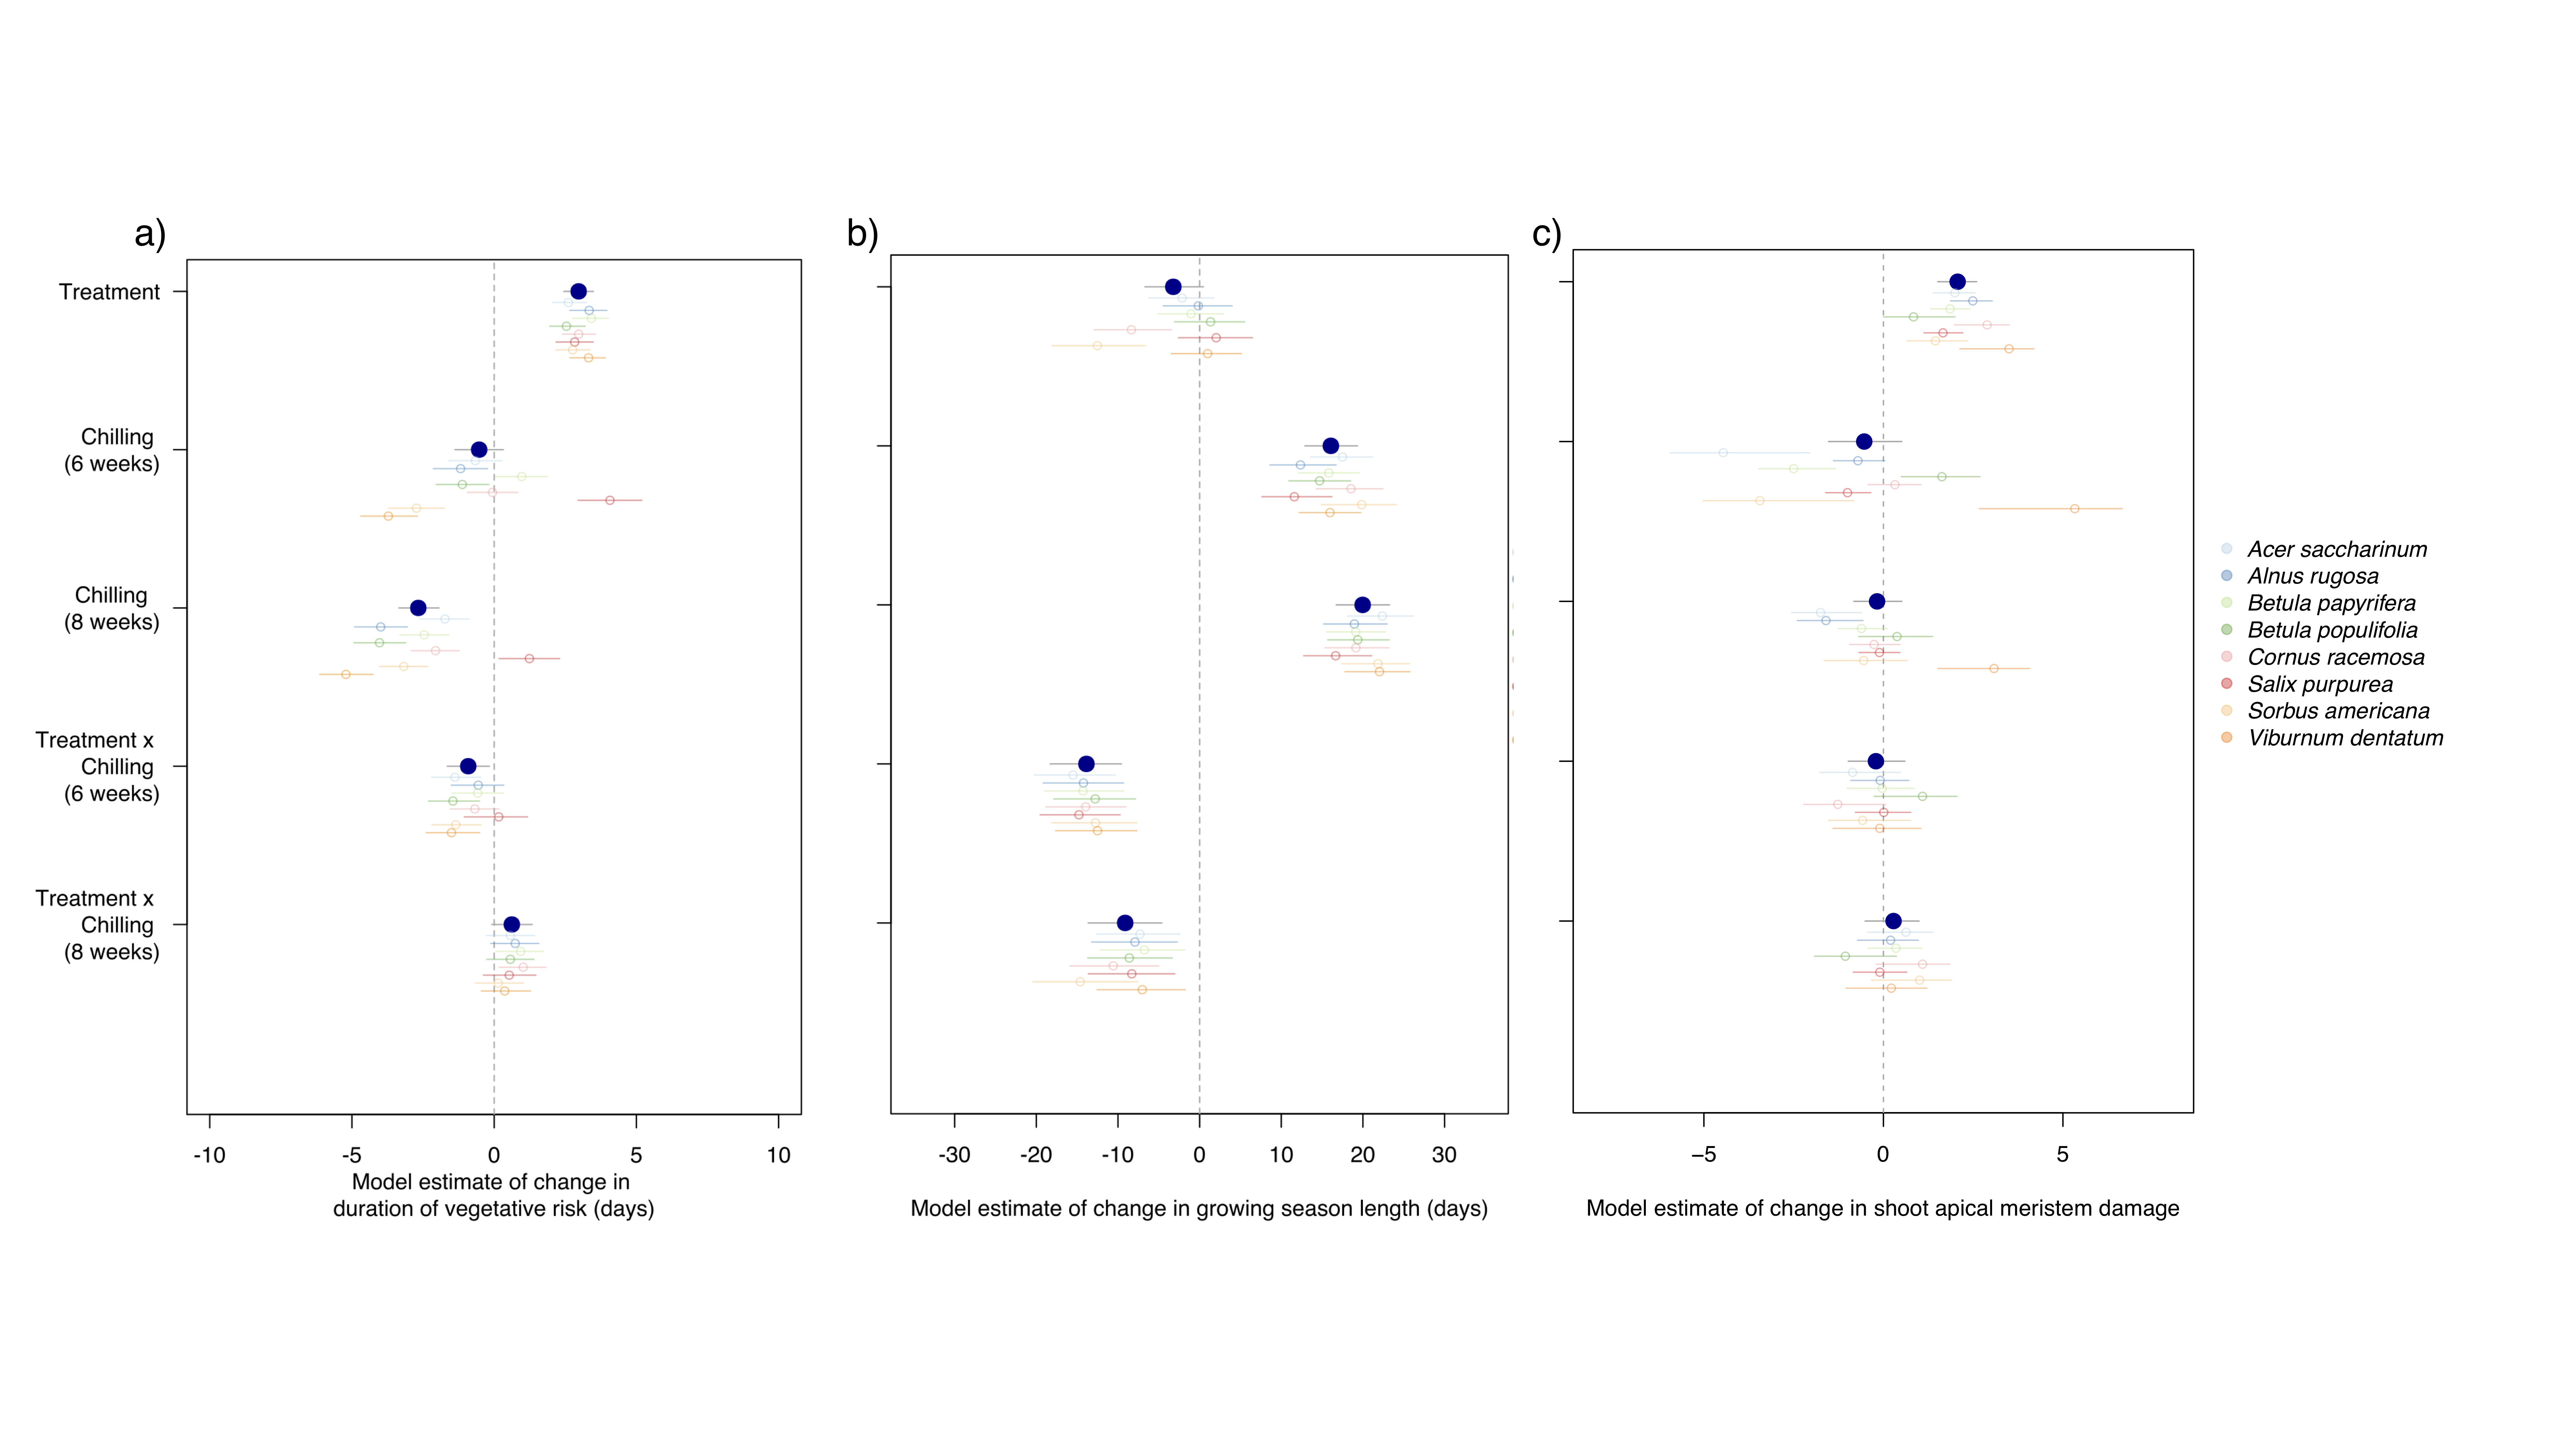
\includegraphics[width=18cm]{..//analyses/figures/mu_phenandmeri.png} %\label{fig:allmsmts}
  -\end{center}
  -\end{figure}}
  
  {\begin{figure} [H]
  -\begin{center}
  -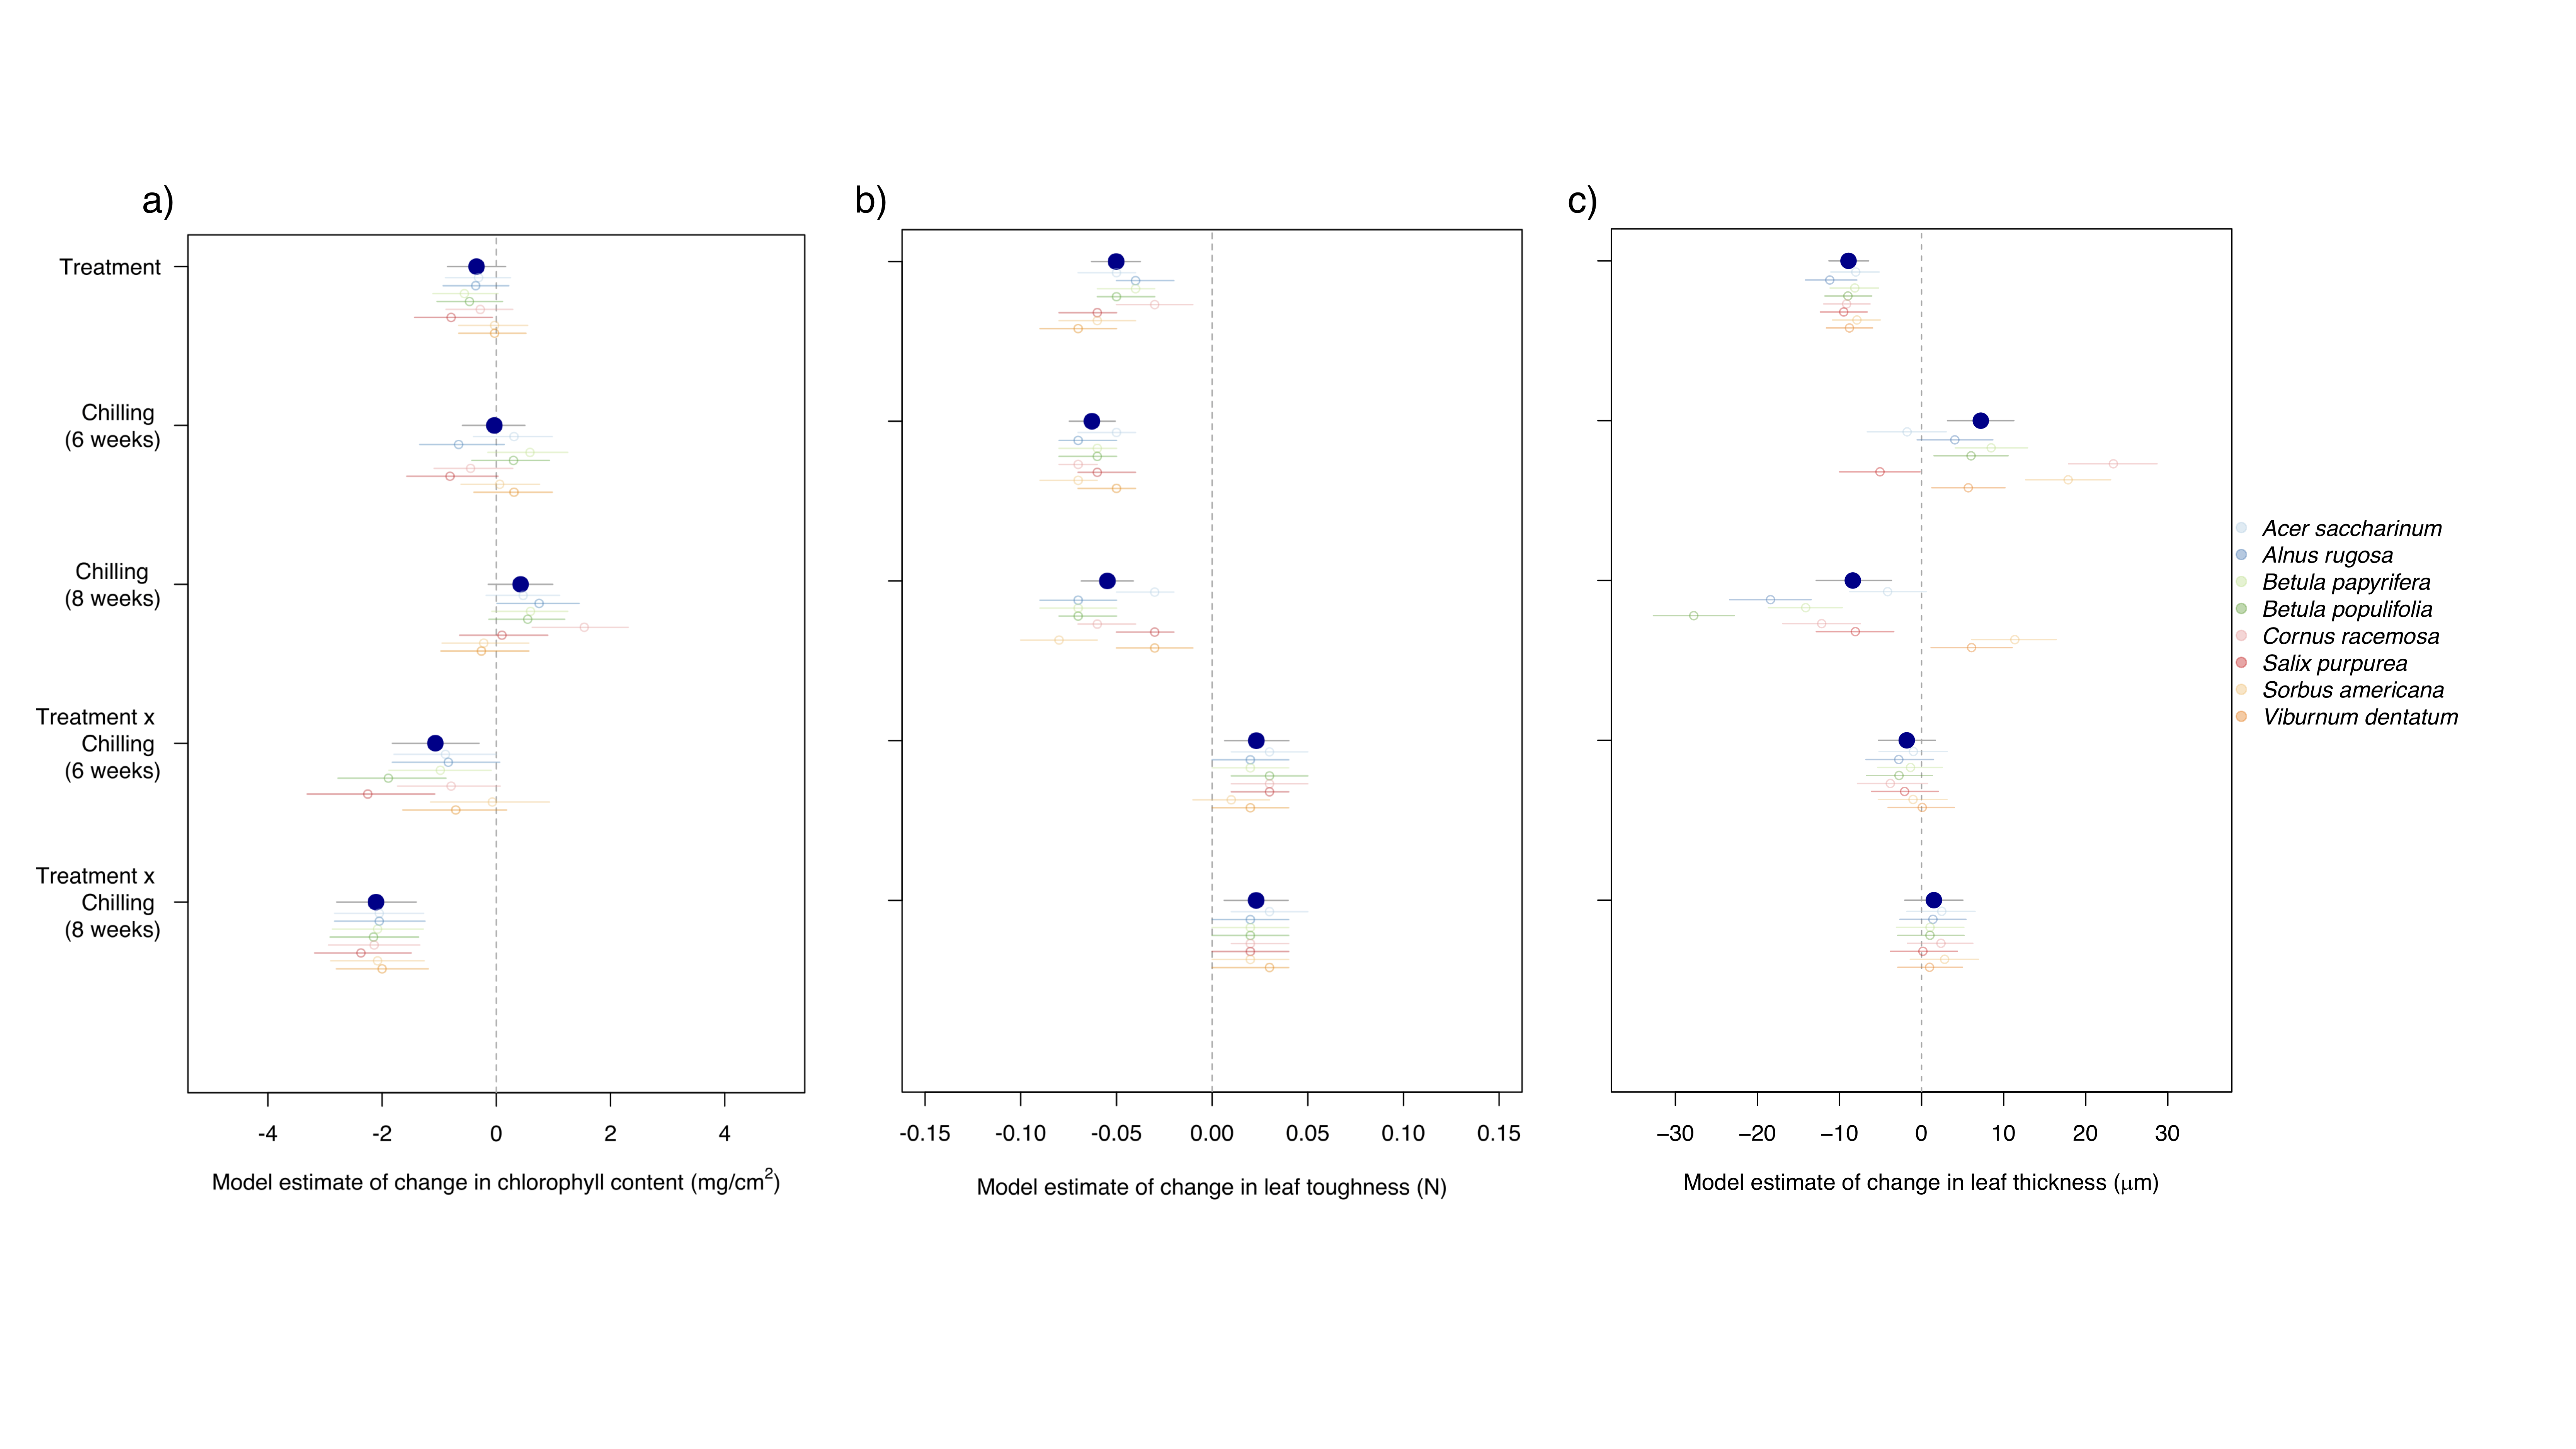
\includegraphics[width=18cm]{..//analyses/figures/mu_leaftraits.png} %\label{fig:allmsmts}
  -\end{center}
  -\end{figure}}
  
  {\begin{figure} [H]
  -\begin{center}
  -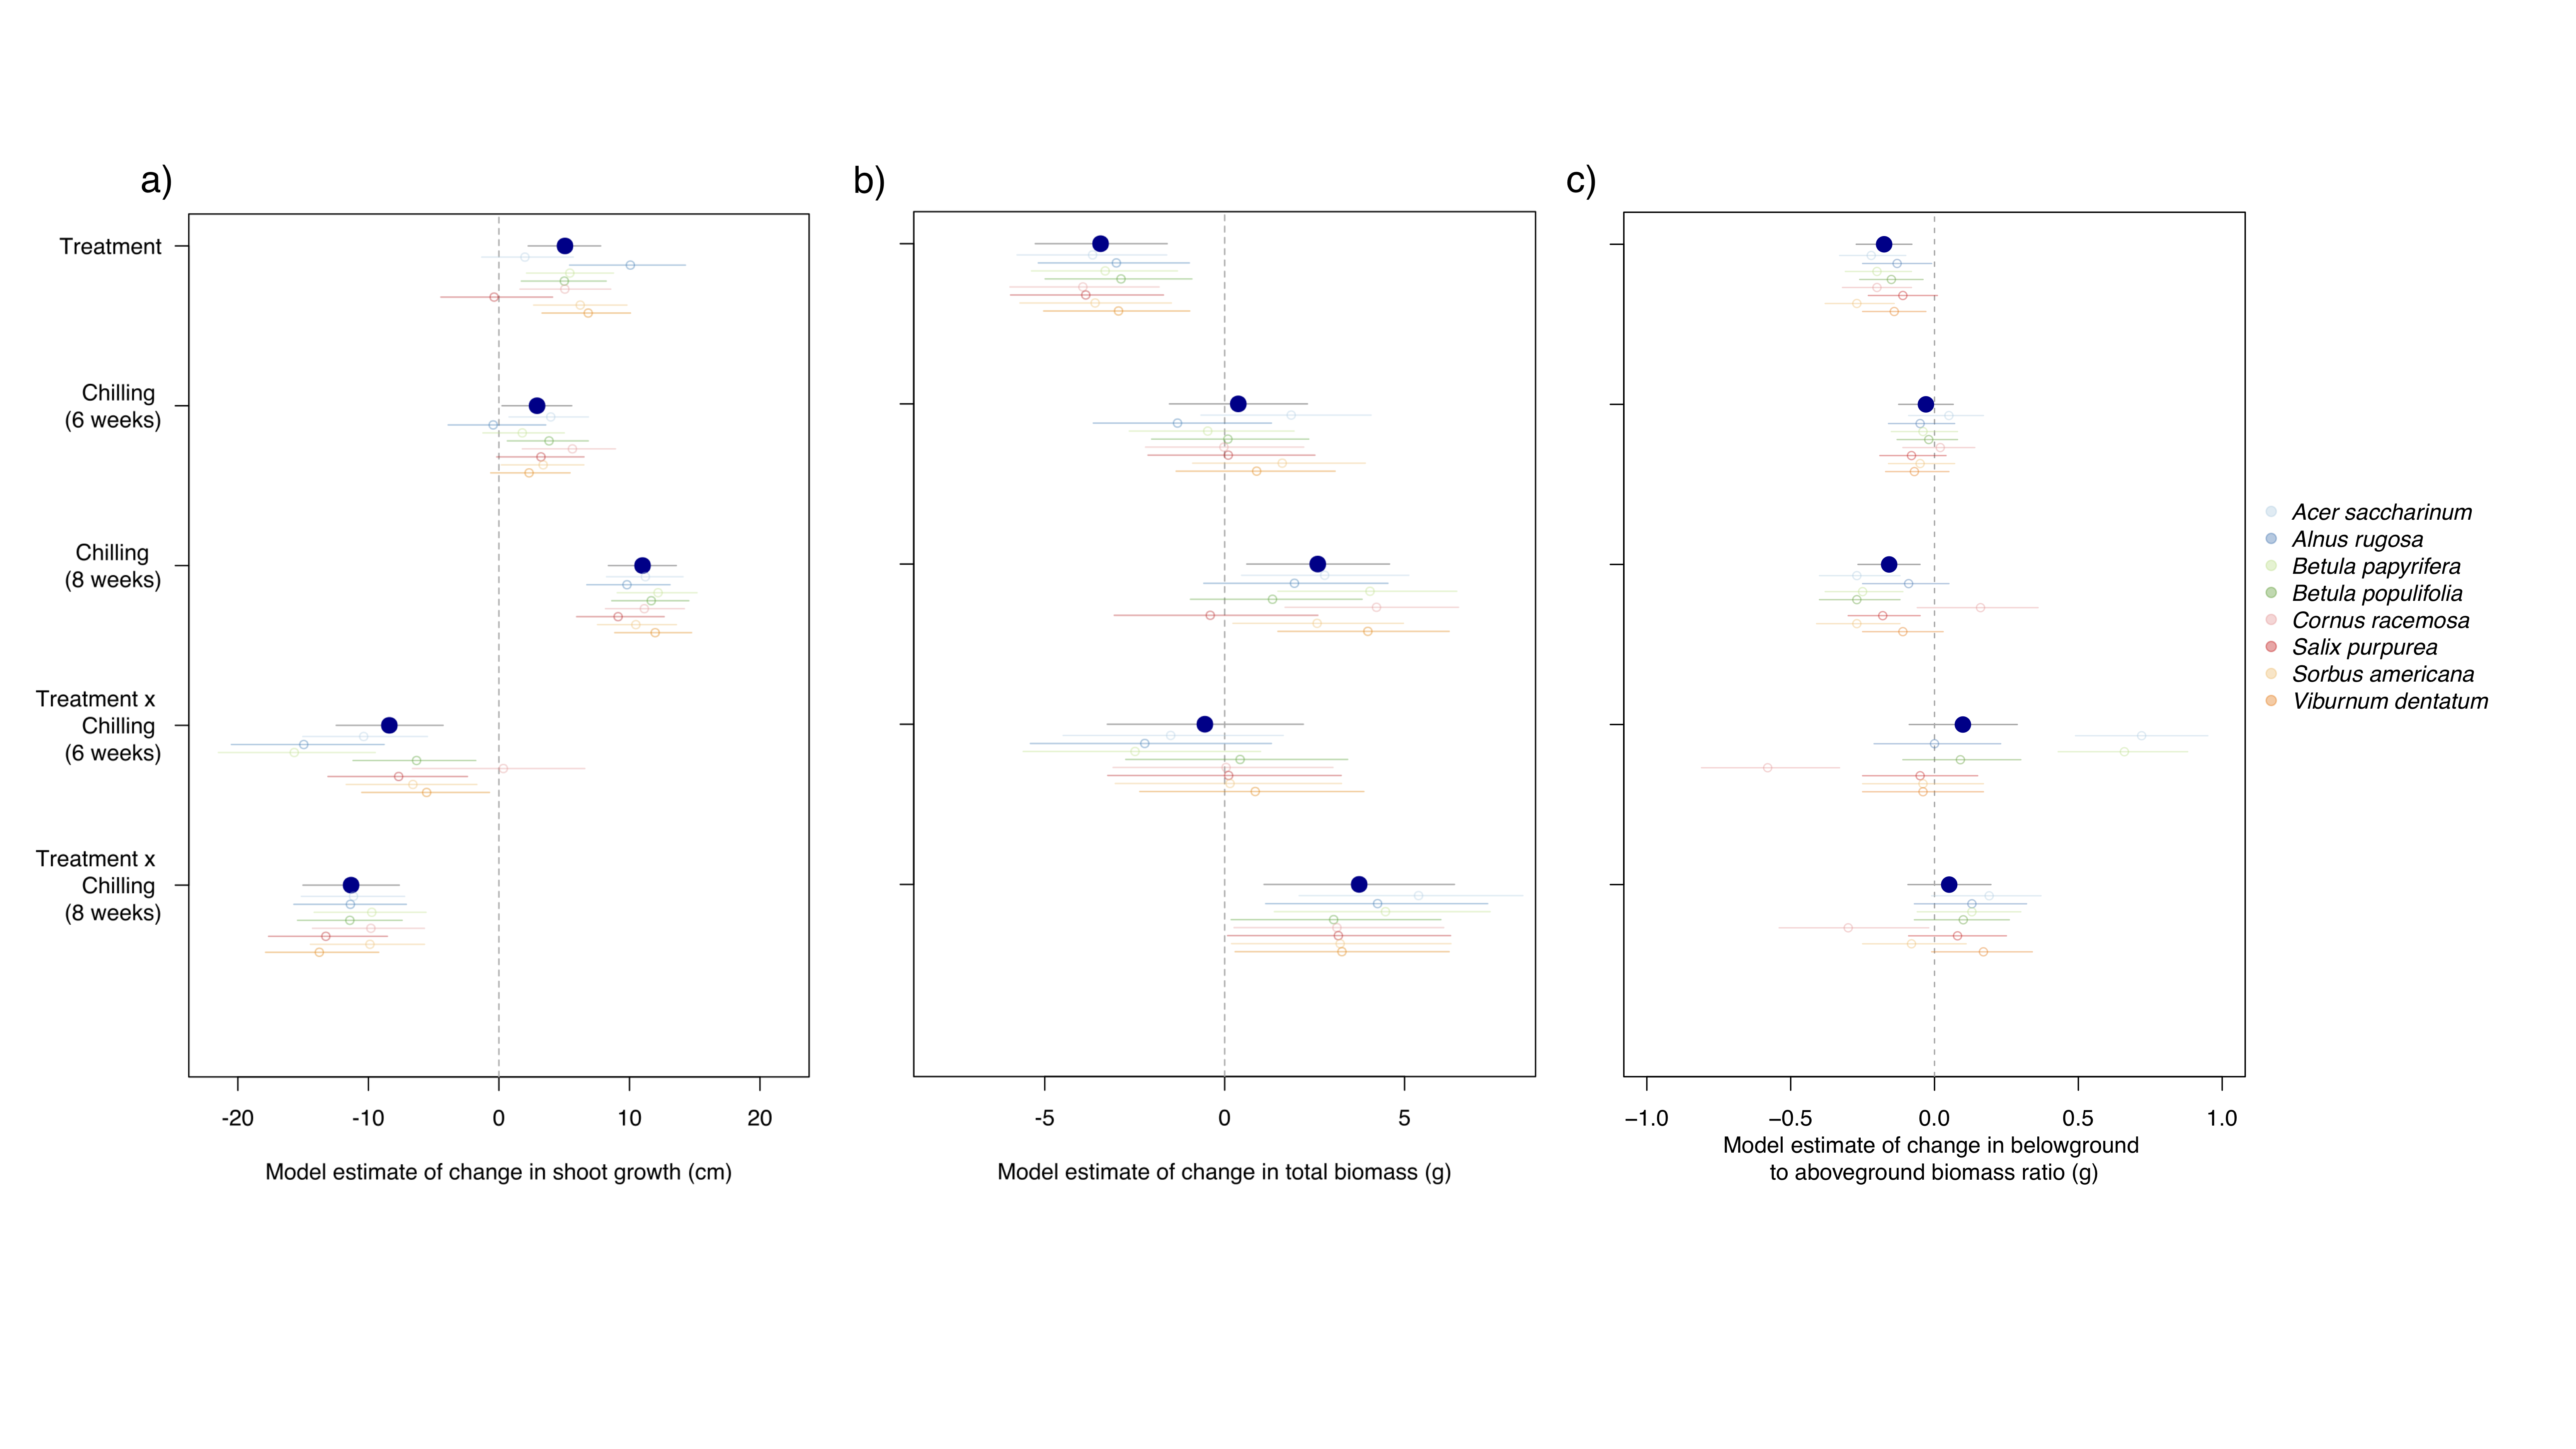
\includegraphics[width=18cm]{..//analyses/figures/mu_growth.png} %\label{fig:allmsmts}
  -\end{center}
  -\end{figure}}
  
  

\end{document}
